\begin{remark}
    Section made from lectures done by Kjellmar Oksavik. Other sources are \citet{BrekkeAsgeir2013Potu} --- chapter 7 parts 6 to 10.
\end{remark}
\section{Auroral particles}
We start with a monoenergetic electron beam \(I_\infty \) at the top of the atmosphere, which will be degraded as it penetrates downward due to collisions with atomic oxygen. The maximum production of the two states will occur when
\begin{equation*}
    \sigma n_{m}H=1
\end{equation*}
where \(\sigma \) is the cross-section and \(n_m\) the density of target atoms at maximum height. When assuming \(H\) to be constant for the density of target atoms, then
\begin{equation*}
    n=n_0\exp\left(-\frac{z}{H}\right)
\end{equation*}
where \(n_0\) is the density of target atoms at \(z=0\). The height of maximum production is then
\begin{equation*}
    z_m=H\ln\left(\sigma n_0H\right)
\end{equation*}
since \(\sigma \{\pres{}{}{O}(\prescript{1}{}{D})\}=10\sigma \{\pres{}{}{O}(\prescript{1}{}{S})\} \), we find
\begin{equation*}
    z_m\{\pres{}{}{O}(\prescript{1}{}{D})\}=z_m\{\pres{}{}{O}(\prescript{1}{}{S})\}+H\ln\left(10\right)
\end{equation*}
The scale height is about 100 km, where the production of the \(\prescript{1}{}{S}\) state has a maximum, is about 7.0 km. The production maximum of the \(\pres{}{}{O}(\prescript{1}{}{D})\) state should then be about 16 km higher according to this simple calculation. In reality, the height difference is greater than this due to quenching at low altitudes and the long lifetime of the state.

\section{Energy deposition profiles of auroral particles}
\(R(\varepsilon_0)\) gives the depth of penetration in a particular medium as a function of the incident particle energy \(\varepsilon_0\). The unit of \(R\) is typically given in \(\tn{g/cm}^2\). The important quantity is not the particle path length but rather the matter traversed by the particle along its path, and this is given by
\begin{equation*}
    N(\ell)=\int_0^\ell n(s)\tn{d}s
\end{equation*}
where \(\ell \) is the point of interest, and \(n(s)\) is the particle density of the matter along the path. For vertical incidence the corresponding function will be
\begin{equation*}
    N(h)=\int_h^\infty n(z)\tn{d}z
\end{equation*}
where \(h\) is the height of interest.

Of course, electron beams are not monoenergetic, but having developed a library of such ionization profiles for a variety of energies within the energy range of interest, composed energy spectra can be used either from measurements or theoretically and more realistic ionization profiles can be derived. For a Maxwell spectra we have
\begin{equation*}
    \phi=\phi_0\varepsilon e^{-\varepsilon/\varepsilon_0}
\end{equation*}
where \(\varepsilon_0\) is the characteristic energy.

\section{Deriving energy spectra from electron density profiles}
In the reverse sense it is possible to retrieve the energy spectrum of precipitating auroral particles if the ionization profile can be measured by, for example, a rocket probe or an incoherent scatter radar. If we assume that a steady state is valid, then the electron production at height \(z\) in the E-region is approximately given by
\begin{equation*}
    q_0(z)=\alpha(z)n_e^2(z)
\end{equation*}
where \(\alpha(z)\) is the recombination coefficient and \(n_e(z)\) is the electron density as a function of height. An observed electron density profile can therefore, when transport terms are neglected and a steady state is assumed, yield the ion-pair production profile to a first approximation. By now applying a library of ionization profiles \(q_i(\varepsilon_i,z)\) derived for a large variety of monoenergetic beams of energy \(\varepsilon_i\), a combination of these profiles should yield the observed ion production profile. Then, assuming we can form a linear combination of \(q_i(\varepsilon_i,z)\) at each discrete height \(z_j\), we have
\begin{equation*}
    q(z_j)=\sum_{i=1}^{N}a_{i}q_i(\varepsilon_i,z_j)
\end{equation*}
where the energy range is \(\varepsilon_1\)--\(\varepsilon_N\) and the number of heights can be chosen arbitrarily. The factor \(a_i\) now represents the weight at which the different monoenergetic energy beams contribute to the total profile.

We apply a least square fit to the deduced ion profile \(q_0(z_j)\)
\begin{equation*}
    \delta=\sum_{j=1}^M{\left[q_0(z_j)-q(z_j)\right]}^2=\sum_{j=1}^M{\left[q_0(z_j)-\sum_{i=1}^{N}a_{i}q_i(\varepsilon_i,z_j)\right]}^2
\end{equation*}
where \(M\) is the number of heights between the lower height \(z_1\) and the upper height \(z_M\). By finding the minimum of \(\delta \) with respect to the coefficients \(\left \{a_j\right \} \) we derive the spectrum.

\subsection{Bremsstrahlung}
An auroral electron emits electromagnetic radiation when it is deflected by Coulomb collisions with atmospheric molecules. This radiation is called ``bremsstrahlung'' and represents a flat continuum in the spectral range \(\nu \) given by
\begin{equation*}
    \nu<\frac{\varepsilon}{h}
\end{equation*}

\section{Excitation processes in the aurora}
One of the best understood auroral emissions is related to excitation of the \(\pres{}{}{N}_2^+\) ion, more specifically to the \(B^2\Sigma_\mu^+\) state which has a maximum cross-section of excitation close to 100 eV. Because they are spontaneous emissions, radiation occurs at the incidence of primary and secondary particles (within \(10^{-7}\) s). Approximately 1 photon at 391.4 nm appears, according to laboratory experiments, to be produced per 50 ion pairs formed in the atmosphere by auroral particles. Therefore, the number of photons resulting from an incident electron with an initial energy \(\varepsilon_0\) can be calculated to be
\begin{equation*}
    \eta(391.4\tn{ nm})=0.02\frac{n(\pres{}{}{N}_2)}{n}\frac{\varepsilon_0}{W}
\end{equation*}
where \(W\) is the mean ionization energy equal to about 35 eV.

The most predominant emission in the high-latitude aurora is the yellow–green line at 557.7 nm. The line is known to be due to the \(\prescript{1}{}{S}\)--\(\prescript{1}{}{D}\) transition in atomic oxygen where the \(\prescript{1}{}{S}\) state has a lifetime against radiation of approximately 0.75 s. Therefore, the transition is so-called forbidden, leaving the oxygen atom long enough in the excited \(\prescript{1}{}{S}\) state for it to be quenched by collisions with other gas particles in the atmosphere.

How the excitation occurs is still not clear, but three ways are possible.
\begin{align*}
    \pres{}{}{O}(\prescript{3}{}{P})+e&\longrightarrow \pres{}{}{O}(\prescript{1}{}{S})+e\qquad\tn{electron impact}\\
    \pres{}{}{O}_2^++e&\overset{k_{\pres{}{}{O}_2^+}}{\longrightarrow} \pres{}{}{O}(\prescript{1}{}{S})+\pres{}{}{O}\qquad\tn{dissociative recombination}\\
    \pres{}{}{N}_2\left(A^2\Sigma\right)+\pres{}{}{O}&\overset{k_{\pres{}{}{N}_2}}{\longrightarrow} \pres{}{}{O}(\prescript{1}{}{S})+\pres{}{}{N}_2\qquad\tn{energy transfer excited }\pres{}{}{N}_2
\end{align*}
For the last two we have delay times given as
\begin{align*}
    \tau_{\pres{}{}{O}_2^+}&=\frac{1}{k_{\pres{}{}{O}_2^+}[\pres{}{}{O}_2^+]}\\
    \tau_{\pres{}{}{N}_2}&=\frac{1}{k_{\pres{}{}{N}_2}[\pres{}{}{N}_2]}
\end{align*}
where the \([\cdot]\) signifies concentrations. What we get from this is that the emissions from 427.8 nm comes before 557.7 nm. This means that the first case, electron impact, cannot be the only process behind the green aurora. In conclusion, all three processes contribute.

Now, let the effective lifetime against radiation for the \(\pres{}{}{O}(\prescript{1}{}{S})\) state be \(\tau \). Then, time variation in the 557.7 nm emission, \(I_{\pres{}{}{O}}(t)\), can be expressed by
\begin{equation}\label{eq:L11_diff_of_oxygen_emission}
    \fracd{I_{\pres{}{}{O}}(t)}+\frac{I_{\pres{}{}{O}}(t)}{\tau}=K_1I_{\pres{}{}{N}}(t)
\end{equation}
where \(I_{\pres{}{}{N}}(t)\) is the intensity of the 427.8 nm emission that is proportional to the production of excited states. Therefore, it is also proportional to the production of the \(\pres{}{}{O}(\prescript{1}{}{S})\) by the proportionality constant \(K_1\), if direct electron impact is the only source. If the 427.8nm emission now exhibits a sinusoidal variation, then we denote
\begin{equation*}
    I_{\pres{}{}{N}}(t)=I_{\pres{}{}{N}_0}e^{i\omega t}
\end{equation*}
Due to the phase lag of the 557.7 nm emission we express
\begin{equation*}
    I_{\pres{}{}{O}}(t)=I_{\pres{}{}{O}_0}e^{i\left(\omega t-\varphi\right)}
\end{equation*}
and find by use of \cref{eq:L11_diff_of_oxygen_emission}
\begin{equation*}
    e^{i\varphi}=\frac{I_{\pres{}{}{O}_0}}{KI_{\pres{}{}{N}_0}}\left(\frac{1}{\tau}+i\omega\right)
\end{equation*}
which then gives
\begin{equation}\label{eq:L11_bad_tan_varphi}
    \tan\varphi=\omega\tau
\end{equation}

Given the frequency of the pulsations, it is therefore possible in principle to derive the effective lifetime \(\tau \) of the upper state of the excited atom related to the 557.7 nm emission. If one performs a cross-spectral analysis of the time signals and derive \(\varphi \) for each frequency component, then there is a linear relationship between \(\omega \) and \(\tan\varphi \) where the slope in the line is represented by the lifetime \(\tau \). The measured \(\tan\varphi \) is not a linear function of \(\omega \) and therefore we conclude the first alternative is not the only mechanism taking place in exciting \(\pres{}{}{O}(\prescript{1}{}{S})\).

Let us therefore include another production term such that
\begin{equation}\label{eq:L11_large_diff}
    \fracd{I_{\pres{}{}{O}}(t)}+\frac{1}{\tau'}I_{\pres{}{}{O}}(t)=K_1'I_{\pres{}{}{N}}(t)+K_2n(t)
\end{equation}
where \(K_2\) is a proportionality constant, the production of \(n(t)\) is proportional to and in phase with the ionization and excitation of the \(\pres{}{}{N}_2^+\) ions emitting the 427.8 nm emission, and the number density decays with a time constant \(\tau_1\)
\begin{equation}\label{eq:L11_n_0_in_large_diff}
    \fracd{n(t)}+\frac{1}{\tau_1}n(t)=K_3I_{\pres{}{}{N}}(t)
\end{equation}

By now assuming the expressions for \(I_{\pres{}{}{N}}(t)\) and \(I_{\pres{}{}{O}}(t)\) and that
\begin{equation*}
    n(t)=n_0e^{i\left(\omega t-\varphi_1\right)}
\end{equation*}
we can solve for both \cref{eq:L11_large_diff,eq:L11_n_0_in_large_diff} and find
\begin{equation}\label{eq:L11_best_tan_varphi}
    e^{i\varphi}=\frac{I_{\pres{}{}{O}_0}}{K_1'I_{\pres{}{}{N}_0}}\frac{\left(\frac{1}{\tau_0}+i\omega\right)\left(\frac{1}{\tau_1}+i\omega\right)}{\frac{1}{\tau_1}+\frac{K_2K_3}{K_1'}+i\omega}
\end{equation}

\Cref{fig_L11_tan_varphi} shows two curves of \(\tan\varphi \) as a function of the frequency observed in a pulsating aurora where there is no linear relationship. Therefore, a least squares fit has been applied to \cref{eq:L11_best_tan_varphi} which appears to correspond better to the observed relationship than \cref{eq:L11_bad_tan_varphi}, indicating that there is a delayed excitation process.
\begin{figure}[t]
    \centering
    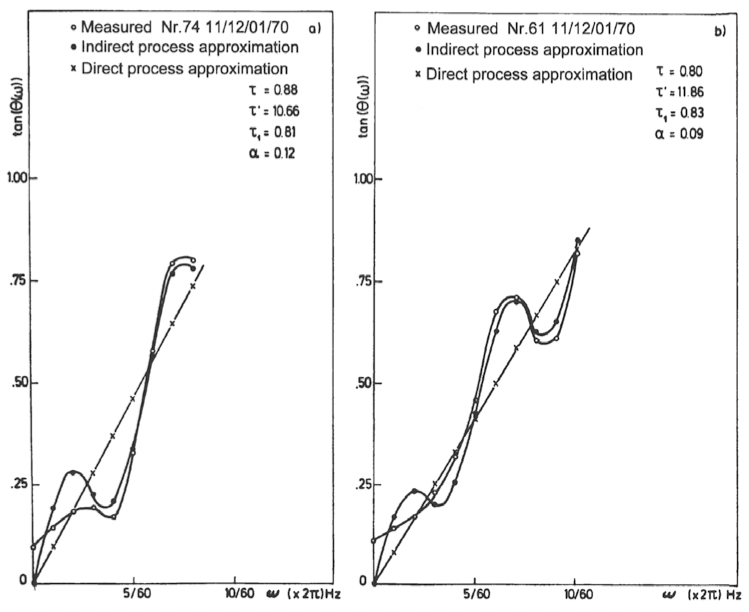
\includegraphics[width=.6\linewidth]{bilder/L11_tan_varphi.png}
    \caption{The tangent of the phase angle \(\varphi \) between the 557.7 nm and 427.8 nm emission as a function of the frequency \(\omega \) as measured in pulsating aurora. (Derived from cross-spectral analysis.)}\label{fig_L11_tan_varphi}
\end{figure}

It turns out that \cref{eq:L11_best_tan_varphi} has two sets of solutions depending on the ratio between \(K_1\) in \cref{eq:L11_diff_of_oxygen_emission} and \(K_1'\) in \cref{eq:L11_large_diff}
\begin{enumerate}[(A)]
    \item If \(K_1'>K_1\) then \(\tau'<\tau_1/\left(1+\tau_1K_2K_3/K_1'\right)\)
    \item If \(K_1'<K_1\) then \(\tau'>\tau_1/\left(1+\tau_1K_2K_3/K_1'\right)\)
\end{enumerate}
which means that if \(K_1'>K_1\) then the effective lifetimes of \(\pres{}{}{O}(\prescript{1}{}{S})\) atoms is always less than the decay time \(\tau_1\) and, in the reverse case, \(\tau'\) may be greater than \(\tau_1\). It is seen that \(\tau_1\) is always larger than \(\tau'\), i.e.\ (A) is what we see in reality.